\documentclass[10pt,preprint]{aastex}
%\usepackage{thumbpdf}
\usepackage{fullpage,amssymb,mathtools}
\usepackage{mathrsfs}
\usepackage{natbib}
\bibliographystyle{apj}

\addtolength{\oddsidemargin}{-.5in}
\addtolength{\evensidemargin}{-.5in}
\addtolength{\textwidth}{0.5in}

\title{Models and Priors Used in 3D Binary Orbit Simulations}
\author{Kyle Mede}
\date{\today}

\begin{document}

\maketitle


% List contents then list of figures
\tableofcontents

\section{Models}
%\section{Description}

These are the outlines of the functions that act as the models to calculate the orbital elements for either a binary star system or planet orbit.  The equations are the result of combining Kepler's laws, the definitions of the orbital elements and the naturally occurring symmetries and rules of a stable binary system.

There are both Python and C++ versions of these functions/models.  The bulk of the multi-process and file management,  post analysis and plotting of the results is done in Python while the computational stages of the simulation are done in C++ to take advantage of its speed.  A more detailed description of these issues and the simulator will be in another document to be written later.




%This function is held in the orbitToolbox2.py toolbox, or library.  This is a collection of functions that are usefull for creating a orbit simulator, such as a basic Monte Carlo or a more complex Markov Chain Monte Carlo simulator.  For a simulator of this type, the inputs to orbitCalculator would be generated using a random number generator, such as random.uniform() in Python.  In this manner, the function would only need to be called each time in the sample loop to provide you the resulting outputs from those random numbers, followed by some type of validity check, such as ensuring the output elements have a chi squared value under a pre-chosen maximum. \\

%This version of the toolbox is for use with the mcmcOrbSimulatorUniform2.py as it uses the input Sep$\_$Angle$\_$Measured$\_$arcsec, Mass1 and Mass2 to find the a1 and a2 values for the system.  The version in the orbitToolbox.py requires a1 and a2 as inputs in order to calculate the output Sep$\_$Angle$\_$Measured$\_$arcsec$\_$model.  The advantage of version 1 is that it calculates a Sep$\_$Angle$\_$Measured$\_$arcsec to compare to the 'real' value measured in the image for chi squared calculations, but it to do this the a1 and a2 parameters must be provided using random numbers.\\

%The function call follows:\\*
%orbitCalculator(t, Sys$\_$Dist$\_$PC, Sep$\_$Angle$\_$Measured$\_$arcsec, inclination$\_$deg, longAN$\_$deg, e, T, period, argPeri$\_$deg, Mass1=1, Mass2=1, verbose=False)\\

%and returns:\\*
%(n, M$\_$deg, E$\_$lates$\_$deg, TA$\_$deg, Sep$\_$Dist$\_$AU$\_$OP, PA$\_$deg$\_$measured$\_$model, a1, a2).

\pagebreak

%----------------------------------------------------------------------------------------------------------------------------------
\subsection{Priors}

In order to include previously determined information about the distribution some of the parameters tend to be for binary systems, sometimes non-uniform priors were used in the Metropolis-Hastings equation for the MCMC simulations.

As found by \citet{duquennoy1991}, for systems with periods$\geq$1000 days, a function of f(e)=2e can be fit to their distribution, else no strong trend was seen.  Thus, we adopt this result and use the normalized prior probability in equation (\ref{eq:eProb1000}) for cases when the period is likely well over 1000days, else a uniform prior is used matching the choice of \citet{gregory2005} for shorter period planets.

\begin{equation}\label{eq:eProb1000}
P_n(e) =  2e
\end{equation}

%\begin{equation}\label{eq:eProb}
%P_n(e) =  \frac{1}{e_{max}-e_{min}}
%\end{equation}
 
To take account for the random possible orbital orientations, a prior proportional to sin(i) is used, (\ref{eq:iProb}).

\begin{equation}\label{eq:iProb}
P_n(i) =  \frac{sin(i)}{cos(i_{min})-cos(i_{max})}
\end{equation}

For situations where the data of the orbit is sparsely sampled, such as in the case of almost all planet and binary systems, one must be careful to avoid aliasing that can lead to a multitude of orbital period solutions.  This effect is thoroughly discussed in \citet{gregory2005}, and the suggestion of using a Jeffreys prior was described as the adequate solution to this problem, (\ref{eq:pProb}).

\begin{equation}\label{eq:pProb}
P_n(P) =  \frac{1}{P ln(\frac{P_{max}}{P_{min}})}
\end{equation}

Assuming the data is gaussian distributed, the rejection function of the Metropolis-Hastings algorithm reduces to (\ref{eq:metHastingsReduced}) once these normalized priors for orbits over 1000days are taken into account.  For those cases where the orbit is well under 1000days, the ratio of the eccentricities simply becomes 1.

\begin{equation}\label{eq:metHastingsReduced}
r(X_t,X_p) = max\bigg\{1, \frac{P_t}{P_p}\frac{e_p}{e_t}\frac{sin(i_p)}{sin(i_t)}e^{\frac{(\chi^2_t - \chi^2_p)}{2}} \bigg\}
\end{equation}

Where, $\chi^2$ is the chi squared fit to the data given by (\ref{eq:chiSquared}).

\begin{equation}\label{eq:chiSquared}
{\chi}^{2} \equiv  \sum_{i=1}^{i=E} \frac{(model_i - observed_i)^{2}}{\sigma^{2}_i}
\end{equation}

\pagebreak
%----------------------------------------------------------------------------------------------------------------
\subsection{True Anomaly Calculator}
The True Anomaly Calculator is used for both models as it is more general.
%\subsubsection{Inputs}

\begin{table}[h]
\centering
\caption{ Inputs to the True Anomaly Calculator.}
\begin{tabular}{c c c}
\hline\hline
Parameter & Description & Typical Range \\
\hline
t* & epoch of observation/image [julian date] & n/a\\
e & eccentricity of orbits [unitless] & [0.001,0.999]\\
T & Last Periapsis Epoch/time [julian date] & [t-period,t]\\
$T_c$* & Last Transit Center Epoch/time [julian date] & [t-period,t]\\
period & period of orbits [yrs] & [1.0,100.0]\\
verbose & Send prints to screen? [True/False](Default = False) & n/a\\
\hline
\end{tabular}
\\
 * = Normally measured/known (ie. not random numbers).
\end{table}

%\subsubsection{Outputs}

\begin{table}[h]
\centering
\caption{ Outputs of the True Anomaly Calculator.}
\begin{tabular}{c c}
\hline\hline
Parameter & Description \\
\hline
n** & Mean Motion [rad/yr] \\
M** & Mean Anomaly [$^{\circ}$]\\
E & Eccentric Anomaly [$^{\circ}$]\\
$\theta$ & True Anomaly [$^{\circ}$]\\
\hline
\end{tabular}
\\
 ** = Not currently returned, but easily could be if needed.
\end{table}

%\subsubsection{Equations}

First calculate the Mean Motion from the provided period:
\begin{equation}\label{eq:4.1.1}
n = \frac{2\pi}{period} 
\end{equation}

Use the Mean Motion, n, time of current epoch(t), time of last periapsis(T), and time of transit center relative to last periapsis (Tc) to get the updated Mean Anomaly:
\begin{subequations}\label{eq:RV-Ma}
\begin{align}
phase& = \frac{Tc-T}{period_{days}} \\
%int\bigg(\frac{Tc-T}{period_{days}}\bigg)period_{days}
\label{eq:RV-Mb}
M& = n \bigg( \frac{(t-T)}{365.25} \bigg)+(phase)2\pi\\
\label{eq:4.1.2}
M& = n \bigg( \frac{(t-T)}{365.25} \bigg)
\end{align}
\end{subequations}
%where 'int()' refers to taking the integer value of what is in the brackets.

The phase of the companion in equation(\ref{eq:RV-Ma}) is unit-less value between 0 and 1.  In equation (\ref{eq:RV-Mb}), the first term is essentially a fraction of how far the current epoch is away from the time of last periapsis multiplied by the Mean Motion throughout the orbit, resulting in units of radians.  The second term involves the unit-less phase converted into radians, thereby having values of 0 and 2$\pi$ at the start and end of each full orbit to match that of the first term.  Following these equations (\ref{eq:4.1.3})-(\ref{eq:4.1.5b}) would be used to calculate the True Anomaly needed in the radial velocity calculations shown below.  This modified version of the Mean Anomaly equation is only needed in the case where the companion transits in front of the primary.  When this does not occur, the value of the Tc is set to T, so the modified version reduces to the original form shown in (\ref{eq:4.1.2}).
It was found that because of the sine function in (\ref{eq:4.1.4}), shifting the phase ahead into a positive value within $2\pi$ cures any issues of angle ambiguity.

The relation between the Eccentric Anomaly, E, and the Mean Anomaly, M, is a transcendental equation and must be solved using numerical methods, shown below.
\begin{equation}\label{eq:4.1.3}
M = E - e\times\sin(E)
\end{equation}
In order to obtain the solution for E the fastest using the Newton's loop and (\ref{eq:4.1.4}), the closest guess of E should be used as the initial value of E$\_$last.
  This also helps to avoid ending up with one of the wrong solutions in the
  cases where there are multiple crossings of the two functions that make up
  equation (\ref{eq:4.1.3}).  A suggested initial guess, that we found to work well, is given by (\ref{eq:4.1.3.5}) as was recommended in \citet{Argyle}.

\begin{equation}\label{eq:4.1.3.5}
E_0 = M+e\sin(M) + \frac{e^2}{2M}sin(2M)
\end{equation}

Newton's method to calculate E:
  
\begin{equation}\label{eq:4.1.4}
E\_latest = E\_last - \frac{[E\_last - e \times \sin(E\_last) - M]}{[1.0 - e \times \cos(E\_last)]}
\end{equation}
The loop completes when E$\_$latest and E$\_$last are the same to 10 decimal places.  It is also checked to ensure it satisfies the original equation (\ref{eq:4.1.3}) with similar precision.  The maximum value of e possible was found to be ~0.98, as precisional rounding issues caused division by zero above this.\\

Use the resultant E$\_$latest to calculate the True Anomaly:
\begin{subequations}
\begin{align}
\label{eq:4.1.5a}
TA& = \arccos \bigg( \frac{[\cos(E\_latest) - e]}{[1.0 - e \times \cos(E\_latest)]} \bigg)\\
\label{eq:4.1.5b}
TA\_true& = \theta = \left\{ \begin{array}{l l} TA& \quad \text{ if E$\_$latest$\leq$ 180$^{\circ}$}\\ 360^{\circ}  - TA& \quad \text{ if E$\_$latest $>$ 180$^{\circ}$} \end{array}\right.
\end{align}
\end{subequations}

Equation (\ref{eq:4.1.5a}) has one unfortunate attribute, as the Eccentric Anomaly grows over $\pi$ (180$^{\circ}$) the resulting value for the True Anomaly goes down, rather than up as should happen.  Thus, to solve this problem the conditional statements of (\ref{eq:4.1.5b}) are applied.\\  
\pagebreak
%----------------------------------------------------------------------------------------------------------------------------------


\subsection{Direct Imaging (Astrometry) Model}
There are two versions of this model, the one used by C++ for the simulation, and the one used by Python in the post processing and plotting.  Both have been checked to ensure the produce the same results for a given set of inputs.  They were chosen to be optimized for each purpose.
%\subsubsection{Inputs}
\begin{table}[h]
\centering
\caption{ Inputs to the Astrometry Model.}
\begin{tabular}{c c c}
\hline\hline
Parameter & Description & Typical Range \\
\hline
t* & epoch of observation/image [Julian date] & n/a\\
Sys$\_$Dist* & measured system distance from Earth [PC] &  [0.01,50.0]\\
$\rho$* & Measured Separation Angle ["] & [0.01,10.0]\\
$\Delta\rho$* & Error in Measured Separation Angle ["] & [0.01,10.0]\\
$\phi$*  & Measured Position Angle  [$^{\circ}$] & [0,360]\\
$\Delta\phi$*  & Error in Measured Position Angle  [$^{\circ}$] & [0,360]\\
{\it i} & inclination [$^{\circ}$] & [0,180]\\
$\Omega$ & Longitude of Ascending Node [$^{\circ}$] & [0,360]\\
$\omega$ & Argument of Periapsis [$^{\circ}$] & [0,360]\\
e & eccentricity of orbits [unitless] & [0.001,0.999]\\
T & Last Periapsis Epoch/time [julian date] & [t-period,t]\\
period & period of orbits [yrs] & [1.0,100.0]\\
a*** & Total Semi-major axis [AU]  & [0.1,200] \\
Mass1*** & Mass of primary star [M$_{\sun}$] & [0.001,10] \\
Mass2*** & Mass of companion [M$_{\sun}$] & [0.001, Mass1] \\
verbose & Send prints to screen? [True/False](Default = False) & n/a\\
\hline
\end{tabular}
\\
 * = Normally measured/known (ie. not random numbers).\\
 *** = Optional.
\end{table}

%\subsubsection{Outputs}

\begin{table}[h]
\centering
\caption{ Outputs of the Astrometry Model.}
\begin{tabular}{c c}
\hline\hline
Parameter & Description \\
\hline
$\chi^{2}_{\nu}$ & Reduced Chi Squared \\
a & Total Semi-major axis [AU]  \\

\hline
\end{tabular}
\end{table}

%\subsubsection{Equations}

If no semi-major axis value is provided, then it is calculated from the period, known masses of the bodies and Kepler's third law:
\begin{equation}\label{eq:28}
a = \bigg[\frac{P^2G(M_1+M_2)}{4\pi^2} \bigg]^{(1/3)}
\end{equation}

The Thiele-Innes method of solving for the orbital elements of binary systems was first found by \citet{Thiele}, and advanced with the inclusion of the Innes constants formulated by \citet{Van}.  This approach has been mainstream ever since, and the equations to find the ephemeris are given below and can be found in \citet{aitken}, \citet{binnendijk} and \citet{heintz}.



\begin{subequations}
\begin{align}\label{eq:24a}
A& = a[cos(\Omega)cos(\omega)-sin(\Omega)sin(\omega)cos(i)]\\
\label{eq:24b}
B& = a[sin(\Omega)cos(\omega)+cos(\Omega)sin(\omega)cos(i)]\\
\label{eq:24c}
F& = a[-cos(\Omega)sin(\omega)-sin(\Omega)cos(\omega)cos(i)]\\
\label{eq:24d}
G& = a[-sin(\Omega)sin(\omega)+cos(\Omega)cos(\omega)cos(i)]
\end{align}
\end{subequations}



The x and y components of the location on the apparent ellipse are found using:
\begin{subequations}
\begin{align}\label{eq:28-1a}
x& = AX+FY\\
\label{eq:28-1b}
y& = BX + GY
\end{align}
\end{subequations}

knowing,

\begin{subequations}
\begin{align}\label{eq:28-1.5a}
X& = \frac{r_j}{a}cos(\theta_j) = cos(E_j)-e\\
\label{eq:28-1.5b}
Y& = \frac{r_j}{a}sin(\theta_j) = \sqrt{1-e^2}sin(E_j) 
\end{align}
\end{subequations}

where, $\theta$ is the True Anomaly, E is the Eccentric Anomaly and r is the distance between the object and the center of mass at a particular time in the orbit.  These are the only equations where the current position through the orbit is taken into account, and it is critical for making the predicted x,y values match the observed ones at a particular epoch (j).

Equations \ref{eq:4.1.1} - \ref{eq:4.1.5b} are used to calculate True Anomaly ($\theta$), Mean Anomaly (M), Eccentric Anomaly (E) and Mean Motion (n); although, because M and n are not needed afterwards, they are not returned at the moment, but could easily be if required.

The respective values from the measured position angle ($\phi$) and separation angle ($\rho$) are:
\begin{subequations}
\begin{align}\label{eq:28-2a}
x& = \rho cos(\phi)\\
\label{eq:28-2b}
y& = \rho sin(\phi)
\end{align}
\end{subequations}

\begin{equation}\label{eq:33}
\chi^{2} \equiv  \sum_{i=1}^{i=E} \frac{(model_i - observed_i)^{2}}{\sigma^{2}_i} = \sum_{i=1}^{i=E} \frac{(x_{model_i}-x_{observed_i}) ^{2}}{\sigma^{2}_{xi}} +\sum_{i=1}^{i=E} \frac{(y_{model_i}-y_{observed_i}) ^{2}}{\sigma^{2}_{yi}}
\end{equation}

\begin{subequations}
\begin{align}\label{eq:reducedChiSquare}
\chi^{2}_{\nu}& \equiv \frac{1}{\nu}\chi^{2}\\
\label{eq:nu}
\nu& \equiv \#\text{observables}-\#\text{free parameters}=2E-(\text{6 OR 7})
\end{align}
\end{subequations}
The "(6 OR 7)" in (\ref{eq:nu}) is due to the option to vary the total semi-major axis, making 7 parameters free, or calculate it from Kepler's third law which reduces the number of free parameters to 6.  There is an option in the code to draw the mass of the two bodies and the system distance from Gaussian distributions centered on the measured values and the variance of those measurements being used as the distribution's variance.  Even though these values are then not fixed, they are not considered free parameters when calculationg $\nu$.
\pagebreak
%----------------------------------------------------------------------------------------------------------------------------------

\subsection{Radial Velocity Model}
%\subsubsection{Inputs}
\begin{table}[h]
\centering
\caption{ Inputs to the Radial Velocity Model.}
\begin{tabular}{c c c}
\hline\hline
Parameter & Description & Typical Range \\
\hline
t* & epoch of observation/image [julian date] & n/a\\
Sys$\_$Dist* & measured system distance from Earth [PC] &  [0.01,50.0]\\
{\it i} & inclination [$^{\circ}$] & [0,180]\\
$\omega$ & Argument of Periapsis [$^{\circ}$] & [0,360]\\
e & eccentricity of orbits [unitless] & [0.001,0.999]\\
T & Last Periapsis Epoch/time [julian date] & [t-period,t]\\
$T_c$* & Last Transit Center Epoch/time [julian date] & [t-period,t]\\
period & period of orbits [yrs] & [1.0,100.0]\\
a*** & Total Semi-major axis [AU]  & [0.1,200] \\
Mass1*** & Mass of primary star [M$_{\sun}$] & [0.001,10] \\
Mass2*** & Mass of companion [M$_{\sun}$] & [0.001, Mass1] \\
K*** & Semi-major Amplitude of primary star [m/s]& [1,500]\\
verbose & Send prints to screen? [True/False](Default = False) & n/a\\
\hline
\end{tabular}
\\
  * = Normally measured/known (ie. not random numbers).\\
 *** = Optional.
\end{table}

%\subsubsection{Outputs}

\begin{table}[h]
\centering
\caption{ Outputs of the Radial Velocity Model.}
\begin{tabular}{c c}
\hline\hline
Parameter & Description \\
\hline
vr & Radial Velocity of primary due to companion [m/s] \\
K & Semi-major Amplitude of primary star [m/s]\\
\hline
\end{tabular}
\end{table}

%\subsubsection{Equations}
In the case of calculating the radial velocity residuals, there are various forms of the equation to calculate predicted radial velocity of the host star due to its companion's motion.

If no semi-major axis value is provided, then it is calculated from the period, known masses of the bodies and Kepler's third law (\ref{eq:28}) and equations (\ref{eq:4.1.10a} - \ref{eq:4.1.10c}).
\begin{equation}\label{eq:28}
a = \bigg[\frac{P^2G(M_1+M_2)}{4\pi^2} \bigg]^{(1/3)}
\end{equation}

The mass ratio can be calculated and used to determine the individual semi-major axis values for each object's orbit as follows:
\begin{subequations}
\begin{align}
\label{eq:4.1.10a}
x& = \frac{Mass2}{Mass1}\\
\label{eq:4.1.10b}
a1& = \frac{a\_total}{1+x}\\
\label{eq:4.1.10c}
a2& = \frac{a1}{x}
\end{align}
\end{subequations}

Equations (\ref{eq:4.1.1} - \ref{eq:4.1.5b}) are used to calculate True Anomaly ($\theta$).

Velocity residual due to a companion star (version used in VRcalcStarStar:VRcalculator):
\begin{equation}\label{eq:30}
vr_s = \bigg[\frac{2\pi G(M_1+M_2)}{P}\bigg]^{1/3}\frac{M_2}{M_1}\frac{sin(i)}{\sqrt{1-e^2}}[cos(\theta+\omega)+e cos(\omega)] = K_s[cos(\theta+\omega)+e cos(\omega)]
\end{equation}

Velocity residual due to a planet around the primary star (version used in VRcalcStarPlanet:VRcalculatorSemiMajorType):
\begin{equation}\label{eq:29}
vr_p = \frac{2\pi a_1sin(i)}{P\sqrt{1-e^2}}[cos(\theta+\omega)+e cos(\omega)]= K_p[cos(\theta+\omega)+e cos(\omega)]
\end{equation}

(Equivalent, but not used currently) Velocity residual due to a planet around the primary star (version used in VRcalcStarPlanet:VRcalculator):
\begin{equation}\label{eq:31}
vr_p = \bigg[\frac{2\pi G}{P}\bigg]^{1/3}\frac{M_2sin(i)}{M_1^{2/3}}\frac{1}{\sqrt{1-e^2}}[cos(\theta+\omega)+e cos(\omega)] = K_p[cos(\theta+\omega)+e cos(\omega)]
\end{equation}

Although, whether $\omega$ is equal to $\omega_1$ or $\omega_2$ is not properly described in \citet{Shulze-Hartung}.  Through personal communications with the author, it was clarified to be $\omega_2$ in all cases.  Following their convention, we set $\omega_1 = \omega_2+\pi$, as it is arbitrary as long as it the convention is mentioned in any resulting research papers.

\begin{equation}\label{eq:33}
{\chi}^{2} \equiv  \sum_{i=1}^{i=E} \frac{(model_i - observed_i)^{2}}{\sigma^{2}_i} = \sum_{i=1}^{i=E} \frac{[(vr_s+vr_p) - (RV_{data}-\gamma)]^{2}}{\sigma^{2}_i}
\end{equation}

where $\gamma $ is the velocity offset of that instrument.  In the case that the velocity of the system's center of mass WRT the Earth has not been removed, the observed component in (\ref{eq:33}) becomes ($RV_{data}-\gamma_{Instrument}-\gamma_{COM}$) (\citet{Paddock} \& \citet{Shulze-Hartung}).  The calculation of $\chi^{2}_{\nu}$ actually occurs outside these functions as the radial velocities due to the companions are calculated separately and then later handled by the higher level function that called the radial velocity model.

%--------------------------------------------------------------------------------------------------------------------------------------

\subsection{Astrometry Models}\label{sec:DI-OrbModels}

\subsubsection{Full Equations Approach}

One method by which to form a model for the apparent ellipse for the orbit of a companion measured with astrometry is to develop them from base equations.  Thus, the equations here are the result of combining Kepler's laws, the definitions of the orbital elements and the naturally occurring symmetries and rules of a stable binary system.\\

First calculate the Mean Motion from the provided period:
\begin{equation}\label{eq:4.1.1}
n = \frac{2\pi}{period} 
\end{equation}

Use the Mean Motion (n), time of current epoch (t) and time of last periapsis (T) to get the Mean Anomaly (M):
\begin{equation}\label{eq:4.1.2}
M = n \bigg( \frac{(t-T)}{365.25} \bigg)
\end{equation}

The relation between the Eccentric Anomaly (E) and the Mean Anomaly is given by Kepler's equation, and is a transcendental equation that must be solved using numerical methods.
\begin{equation}\label{eq:4.1.3}
M = E - {\it e}\times\sin(E)
\end{equation}
In order to obtain the solution for E the fastest using the Newton's loop and (\ref{eq:4.1.4}), the closest guess of E should be used as the initial value of E$^{\prime}$.  This also helps to avoid ending up with one of the wrong solutions in cases where there are multiple crossings of the two functions that make up Equation (\ref{eq:4.1.3}).  A suggested initial guess that we found to work well is given by (\ref{eq:4.1.3.5}), found by \citep{Argyle}.

\begin{equation}\label{eq:4.1.3.5}
E_0 = M+{\it e}\sin(M) + \frac{e^2}{2M}sin(2M)
\end{equation}

Newton's method to calculate E is then given by repeatedly calculating (\ref{eq:4.1.4}) in a loop:
  
\begin{equation}\label{eq:4.1.4}
E^{\prime \prime} = E^{\prime} - \frac{[E^{\prime} - {\it e} \times \sin(E^{\prime}) - M]}{[1.0 - {\it e} \times \cos(E^{\prime})]}
\end{equation}
The loop completes when {\it E$^{\prime \prime}$} and {\it E$^{\prime}$} are the same to 10 decimal places.  It is also checked to ensure the resulting value for {\it E} satisfies the original Equation (\ref{eq:4.1.3}) with the same precision.  The maximum value of {\it e}possible was found to be ~0.98, as rounding issues caused a division by zero above this.\\

Using the resultant {\it E} the True Anomaly ($\theta$) can be calculated following:
\begin{subequations}
\begin{align}
\label{eq:4.1.5a}
\theta^{\prime}& = \cos^{-1} \bigg( \frac{[\cos(E) - e]}{[1.0 -{\it e}\times \cos(E)]} \bigg)\\
\label{eq:4.1.5b}
\theta& = \left\{ \begin{array}{l l} \theta^{\prime}& \quad \text{ if E $\leq$ 180$^{\circ}$}\\ 360^{\circ}  - \theta^{\prime}& \quad \text{ if E $>$ 180$^{\circ}$} \end{array}\right.
\end{align}
\end{subequations}
Equation (\ref{eq:4.1.5a}) has the unfortunate attribute that as the Eccentric Anomaly grows over 180$^{\circ}$, the resulting value for the True Anomaly goes down, rather than up as should happen.  This problem is rectified by applying the conditional statements of (\ref{eq:4.1.5b}).\\  

The pictorial representation of these three anomalies is summarized in Figure \ref{fig:Anomalies}.

\begin{figure}[ht]
\begin{center}
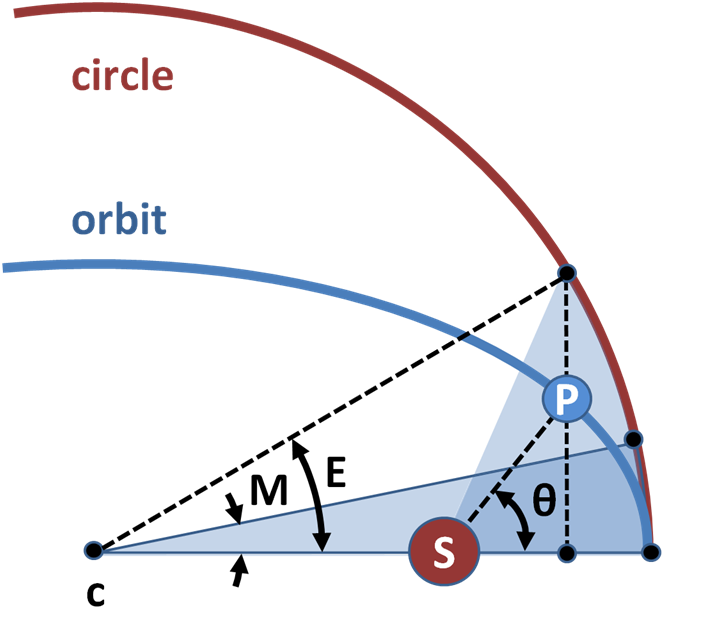
\includegraphics[scale=0.4]{Anomalies-MOD.png}
\caption[Diagram of Anomalies]{A diagram to compare the Eccentric, Mean and True anomalies of an orbiting planet.  The planet is marked as P, the central is S, and the center of the ellipse is C in this plot. }
\label{fig:Anomalies}
\end{center}
\end{figure}

The True Anomaly can then be used to find the Separation Distance in the orbital plane ($R^{\prime}$), split that into its X and Y components (WRT Line of Nodes) in the reference plane.  Pythagoras Theorem can combine these to get final radial Separation Distance in the reference plane ($R$):
\begin{subequations}
\begin{align}
\label{eq:4.1.6a}
R^{\prime}& = \frac{[(a)\times(1-e^{2})]}{[1.0 +{\it e}\times \cos(\theta)]}\\
\label{eq:4.1.6b}
R_y& = R^{\prime} \times \sin(\omega + \theta) \times \cos(i)\\
\label{eq:4.1.6c}
R_x& = R^{\prime} \times \cos(\omega + \theta)\\
\label{eq:4.1.6d}
R& = [(R_y)^{2} + (R_x)^{2}]^{1/2}
\end{align}
\end{subequations}
This method is required as the inclination only affects the y-component in this coordinate system.

Now to find the angle between the Line of Nodes and the secondary body ($\psi$), corrected for inclination:
\begin{subequations}
\begin{align}
\label{eq:4.1.7a}
\psi^{\prime \prime}& = \omega + \theta \text{ , in the orbital plane}\\
\label{eq:4.1.7b}
\psi^{\prime}& = \tan^{-1} \bigg( \frac{R_y}{R_x} \bigg) \text{ , in the reference plane}\\
\label{eq:4.1.7c}
\psi& = \left\{ \begin{array}{l l l} \psi^{\prime}& \quad \text{ if in quadrant 1}\\ \psi^{\prime} + 180^{\circ}& \quad \text{ if in quadrants 2 or 3}\\ \psi^{\prime} + 360^{\circ}& \quad \text{ if in quadrant 4} \end{array}\right.
\end{align}
\end{subequations}
Equation (\ref{eq:4.1.7b}) results in an angle from the X-axis (Line of Nodes) to where M2
is located, rather than from the positive X-axis in a clockwise direction in all
cases.  Thus, it is not always in the quadrant which M2 lies in on a X (Line of Nodes, positive to right in reference plane) Y ($\bot$ to Line of Nodes, positive upwards in the reference plane) grid.  In fact, the resultant angle will be negative for all but the first quadrant.  The four quadrant options are corrected using the conditionals in Equation (\ref{eq:4.1.7c}).\\

The final measured Position Angle only depends on if the sum of all corrected angles in the reference plane sum to more than 360$^{\circ}$ or not, so:
\begin{equation}\label{eq:4.1.8}
\phi= \left\{ \begin{array}{l l} \Omega + \psi& \quad \text{ if sum $\le$ 360$^{\circ}$}\\ \Omega + \psi - 360^{\circ}& \quad \text{ if sum $>$ 360$^{\circ}$}\\ \end{array} \right.
\end{equation}

Lastly, calculate the measured Separation Angle in [$\arcsec$], using the calculated separation distance in the reference plane, in [AU], and the provided system distance (S), in [PC]:
\begin{equation}\label{eq:4.1.9}
\rho= \frac{R}{S}
\end{equation}

For the case where the system is a star and planet, then the previously found {\it a} is approximately the semi-major axis of the planet's orbit, due to $M_1\gg M_2$.  Else, the mass ratio can be calculated and used to determine the individual semi-major axis values for each star's orbit as follows:
\begin{subequations}
\begin{align}
\label{eq:4.1.10a}
x& = \frac{M_2}{M_1}\\
\label{eq:4.1.10b}
a_1& = \frac{a}{1+x}\\
\label{eq:4.1.10c}
a_2& = \frac{a_1}{x}
\end{align}
\end{subequations}

\pagebreak




%-----------------------------------------

\subsubsection{Thiele-Innes Method}\label{sec:TH_I} 

The Thiele-Innes method to solve for the orbital elements of binary systems was first described in \citet{Thiele}, and later advanced with the inclusion of the Innes constants formulated in \citet{Van}.  This approach has been mainstream ever since, and the equations to find the ephemeris are given below can be found in many text books, such as \citet{aitken}, \citet{binnendijk} and \citet{heintz}.

\begin{subequations}
\begin{align}\label{eq:24a}
A& = a[\cos(\Omega)\cos(\omega)-\sin(\Omega)\sin(\omega)\cos(i)]\\
\label{eq:24b}
B& = a[\sin(\Omega)\cos(\omega)+\cos(\Omega)\sin(\omega)\cos(i)]\\
\label{eq:24c}
F& = a[-\cos(\Omega)\sin(\omega)-\sin(\Omega)\cos(\omega)\cos(i)]\\
\label{eq:24d}
G& = a[-\sin(\Omega)\sin(\omega)+\cos(\Omega)\cos(\omega)\cos(i)]
\end{align}
\end{subequations}


From these constants, we then extract the orbital elements in the following way.  First the values for $\omega+\Omega$ and $\omega-\Omega$ are found using:

\begin{subequations}
\begin{align}\label{eq:25a}
\tan(\omega+\Omega)& = \frac{B-F}{A+G} \\
\label{eq:25b}
\tan(\omega-\Omega)& = \frac{-B-F}{A-G}\\
\label{eq:25c}
Angle& = \left\{ \begin{array}{l l l} Angle^{\prime}& \quad \text{ if in quadrant 1}\\ Angle^{\prime} + \pi& \quad \text{ if in quadrant 2 or 3}\\ Angle^{\prime} + 2\pi& \quad \text{ if in quadrant 4}  \end{array} \right.
\end{align}
\end{subequations}

Where the resulting `angle' of $\omega+\Omega$ or $ \omega-\Omega$ from equations (\ref{eq:25a} \& \ref{eq:25b}) are corrected for which quadrant they lie in, determined from the resulting angle's sign and that of the numerator (ie. the sine component), using the conditionals of (\ref{eq:25c}).  These corrected angles can be combined to find the values of 2$\Omega$ and 2$\omega$, then simply dividing by 2 solves for each of the raw form of these values.  Following the standard convention that $\Omega$ lies between $0^{o}-180^{o}$, else, $180^{o}$ should be added to (or subtracted from) both the $\omega$ and $\Omega$ raw values \citep{aitken}.  This convention can be verified by the use of radial velocity data, as discussed in Section \ref{sec:BinaryOrbElements}.

\begin{equation}\label{eq:26}
i = 2\tan^{-1}\bigg(\frac{(A-G)\cos(\omega+\Omega)}{(A+G)\cos(\omega-\Omega)}  \bigg)\\
\end{equation}

\begin{equation}\label{eq:27}
a = \frac{B-F}{2\sin(\omega+\Omega)\cos^2(\frac{i}{2})}
\end{equation}
In the case of a binary star system, the astrometric positions refer to that of the secondary with respect to the primary, rather than the center of mass for the system.  Thus, \citet{Shulze-Hartung} conclude that the output $\omega$ is that of $\omega_2$+$\pi$, and that it equals $\omega_1$ in the case of a planetary system.  They also discuss that the semi-major axis found is that of $a_1+a_2$ when investigating binary stars and simply $a_1$ when investigating planets, see Section \ref{sec:omegaIssues} for more detail on this.

Then using Kepler's third law, the period can be calculated from the semi-major axis value.
\begin{equation}\label{eq:28}
P = \bigg[\frac{4\pi^2a^3}{G(M_1+M_2)} \bigg]^{(1/2)}
\end{equation}

The x and y components of the location on the apparent ellipse are found with:
\begin{subequations}
\begin{align}\label{eq:28-1a}
x& = AX+FY\\
\label{eq:28-1b}
y& = BX + GY
\end{align}
\end{subequations}

knowing,

\begin{subequations}
\begin{align}\label{eq:28-1.5a}
X& = \frac{r_j}{a}\cos(\nu_j) = \cos(E_j)-e\\
\label{eq:28-1.5b}
Y& = \frac{r_j}{a}\sin(\nu_j) = \sqrt{1-e^2}\sin(E_j) 
\end{align}
\end{subequations}
where, $\nu$ is the True Anomaly, E is the Eccentric Anomaly and r is the distance between the object and the center of mass at a particular time in the orbit.  These are the only equations where the current position in the orbit is taken into account, and it is critical for making the predicted x, y values match the observed ones at a particular epoch (j).

Equations (\ref{eq:4.1.1} - \ref{eq:4.1.5b}) are then used to calculate the epoch dependant values: the True Anomaly ($\theta$), Mean Anomaly (M), and Eccentric Anomaly (E).

The respective x and y values from the measured position angle ($\phi$) and separation angle ($\rho$) are given by:
\begin{subequations}
\begin{align}\label{eq:28-2a}
x& = \rho \cos(\phi)\\
\label{eq:28-2b}
y& = \rho \sin(\phi)
\end{align}
\end{subequations}

The error in the data values in the new coordinate system would then be:

\begin{subequations}
\begin{align}\label{eq:28-3a}
\sigma_{x}=\Delta x& = x \sqrt{\bigg(\frac{\Delta\rho}{\rho}\bigg)^2 +\bigg(\frac{\cos(\phi+\Delta\phi)-\cos(\phi)}{\cos(\phi)}\bigg)^2} = \sqrt{(\Delta \rho \cos(\phi))^2+(\rho \sin(\phi)\Delta \phi)^2}\\
\label{eq:28-3b}
\sigma_{y}=\Delta y& = y \sqrt{\bigg(\frac{\Delta\rho}{\rho}\bigg)^2 +\bigg(\frac{\sin(\phi+\Delta\phi)-\sin(\phi)}{\sin(\phi)}\bigg)^2} = \sqrt{(\Delta \rho \sin(\phi))^2+(\rho \cos(\phi)\Delta \phi)^2}
\end{align}
\end{subequations}
 
Both of these calculation methods are equal, ensuring $\phi$ is in [rads] and $\rho$ is in [$\arcsec$].

The orientation and definition of x and y depends on the choice of view of the binary system.  The two most common of these are the telescope and the naked eye view, seen in Figure \ref{fig:4}.  In this figure it can be seen that in the telescope view actually has its North axis being matched to the standard ``y" axis of a Cartesian coordinate system, and East matched to the ``x" axis; due to the fact that the Thiele-Innes Method is based on the Cartesian coordinate system, instead of the `naked eye' or `telescope' views.  So, that if the Cartesian coordinates was rotated by a -90$^\circ$ the x and y axis would match the orientation shown in Figure \ref{fig:4}, with E=y and N=x.  Moving the in opposite direction and rotating by +90$^\circ$ would match the naked eye view, again with E=y and N=x.  Therefore, as long as the measured $\theta$ from the data has the values displayed in the two views of Figure \ref{fig:4}, the equations for the calculated x and y shown above, (\ref{eq:28-2a} \& \ref{eq:28-2b}), will work.


\begin{figure}[ht]
\begin{center}
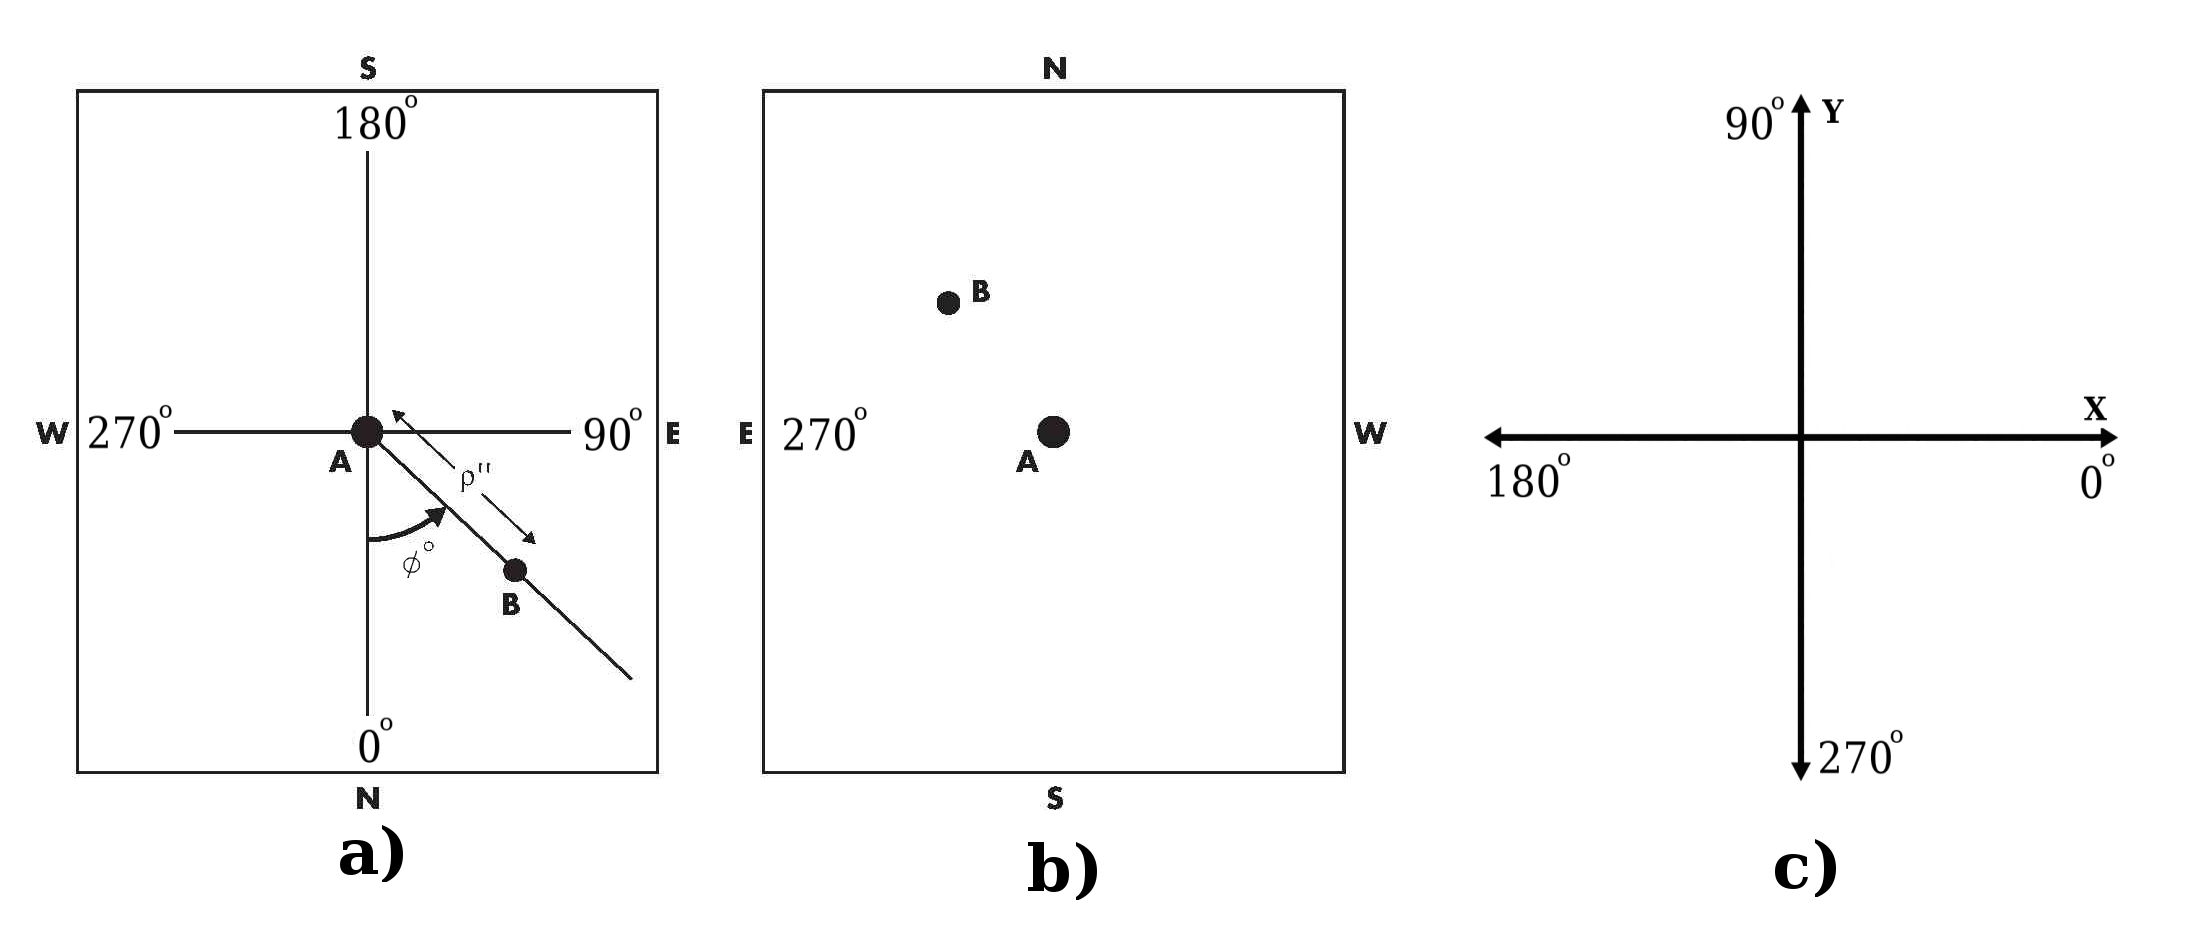
\includegraphics[scale=0.9]{Figures/Argyle-oribit-plots1-cropped-AND-cartesianCoordsPlot.jpg}
\caption[View of a Binary System]{ View of a binary system through a) A telescope, and b) The naked eye, both compared to c) 2D Cartesian coordinate system. \citet{Argyle}. }
\label{fig:4}
\end{center}
\end{figure}

%\begin{figure}[ht]
%	\begin{minipage}{0.45\hsize} %left picture
 %   \begin{center}
 %   \includegraphics[scale=0.7]{Figures/Argyle-oribit-plots1-cropped.jpg}
 %   \end{center}
 %   \caption[View of a Binary System]{ View of a binary system through a. A telescope, and b. The naked eye, %			\citet{Argyle}. }
%    \label{fig:4}
%  \end{minipage}
%  \begin{minipage}{0.4\hsize} %right picture
%    \begin{center}
%    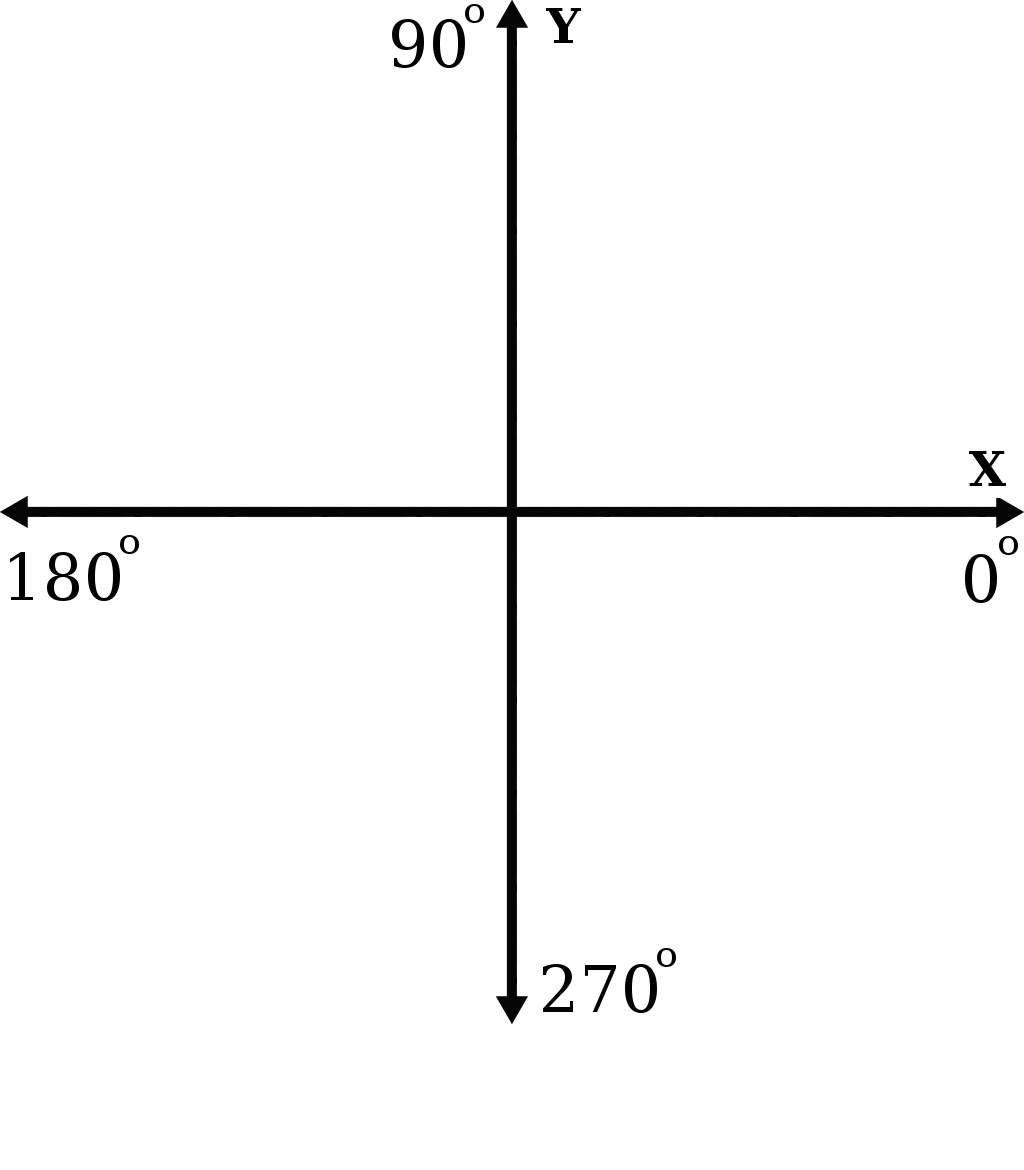
\includegraphics[scale=0.18]{Figures/CartesianCoordSystem-mine2.jpeg}
%    \end{center}
 %   \caption{2D Cartesian coordinate system.}
%    \label{fig:4.5}
%  \end{minipage}  
%\end{figure}


\begin{figure}[ht]
\begin{center}
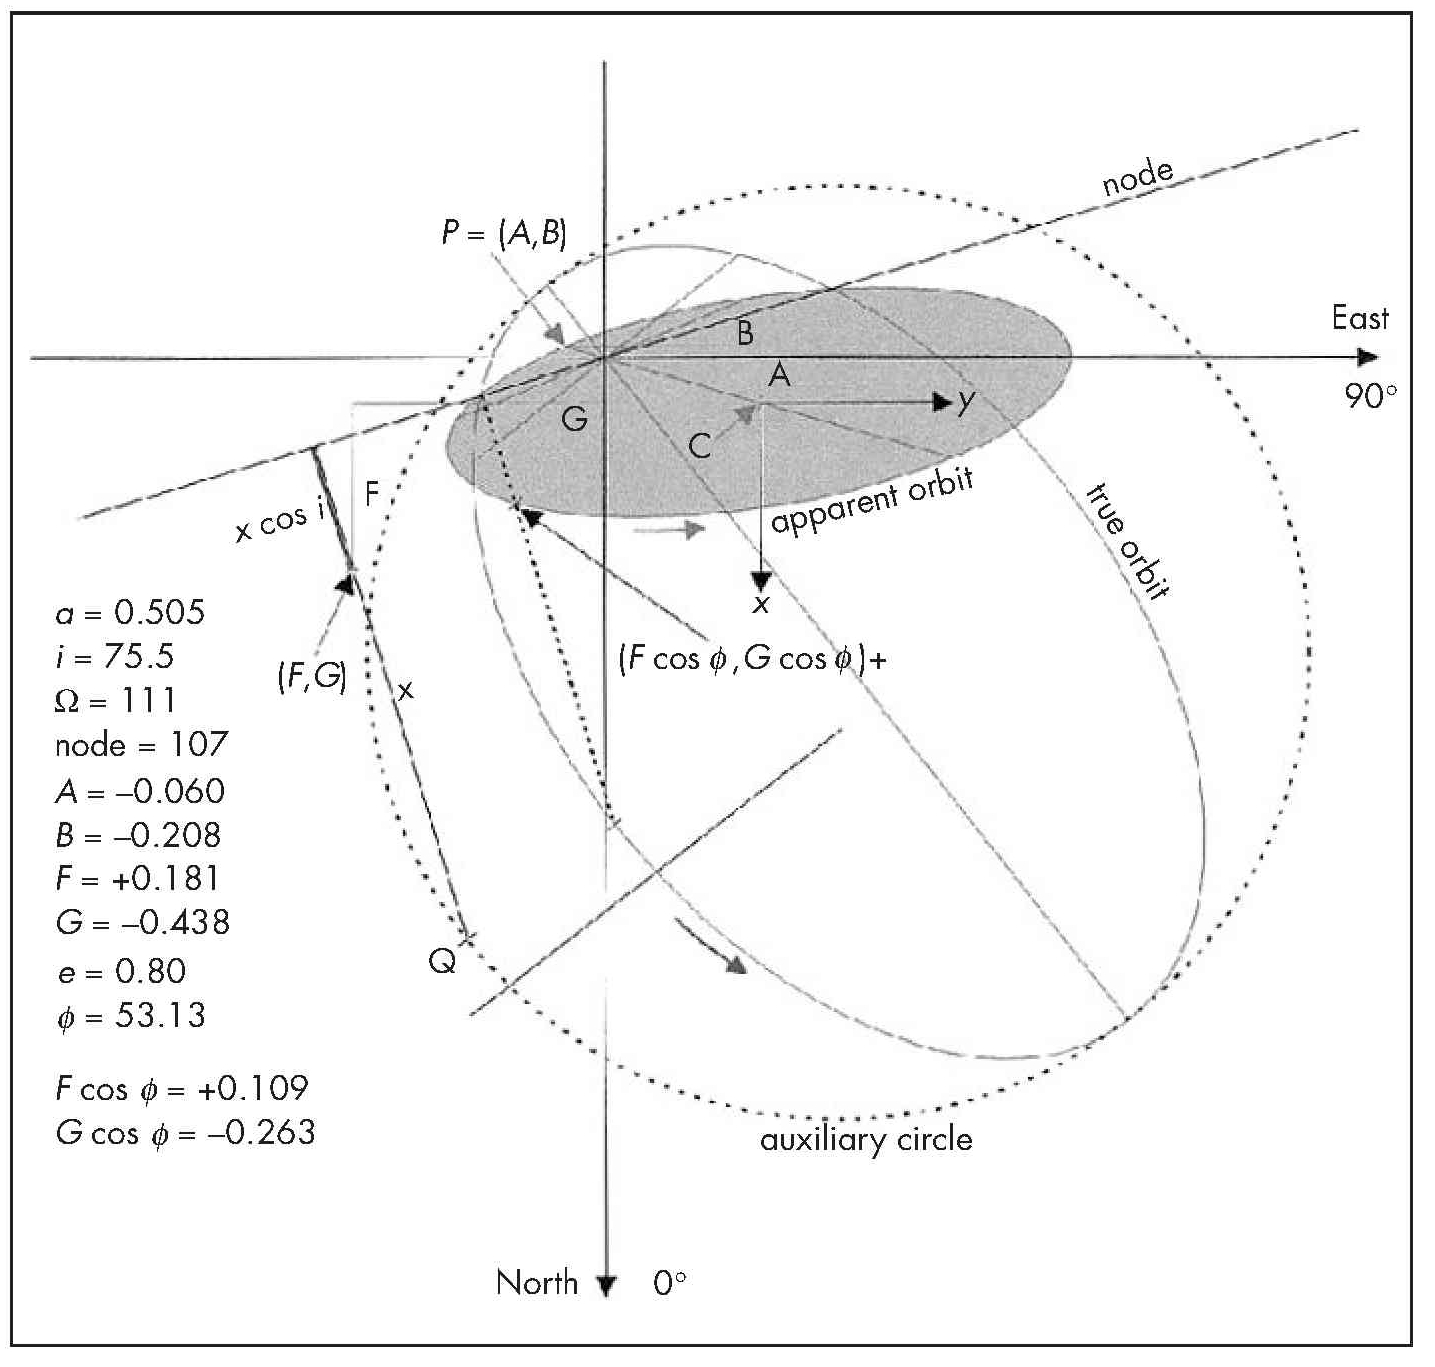
\includegraphics[scale=0.9]{Figures/Argyle-oribit-plots2-cropped.jpg}
\caption[Apparent and True orbital ellipses]{ Plot of apparent and true orbital ellipses, and the Thiele-Innes elements, \citet{Argyle}. }
\label{fig:apparentTrueEllipses}
\end{center}
\end{figure}

In the case where the data is measured as the difference in Right Ascension ($\alpha$) and Declination ($\delta$) of the companion from the primary star, in units of [$\arcsec$], these match the E=y and N=x respectively.  This allows for direct comparison of the data to the values calculated in equations  (\ref{eq:28-1a}) and (\ref{eq:28-1b}).  If these units need to be converted to $\phi$ and $\rho$, then the following conversions can be used.

\begin{subequations}
\begin{align}\label{eq:RADECtoPA}
\phi =&   \tan^{-1}\bigg(\frac{\alpha}{\delta} \bigg)\\
\label{eq:RADECtoSA}
\rho =&   \sqrt{\delta^2+\alpha^2}
\end{align}
\end{subequations}

The conditionals below are needed to correct the resulting angle from (\ref{eq:RADECtoPA}) for all four quadrants.

\begin{equation}\label{eq:4.1.PAcorrection}
\phi_{corrected} = \left\{ \begin{array}{l l l} \phi& \quad \text{ if in quadrant 1}\\ \phi + \pi& \quad \text{ if in quadrant 2 or 3}\\ \phi + 2\pi& \quad \text{ if in quadrant 4}  \end{array} \right.
\end{equation}

\begin{subequations}
\begin{align}\label{eq:RADECtoPAerr}
\Delta\phi =&   \frac{\bigg(\frac{\alpha}{\delta}\bigg) \sqrt{\bigg( \frac{\Delta\alpha}{\alpha} \bigg)^2 \bigg( \frac{\Delta\delta}{\delta} \bigg)^2} }{1.0+\bigg(\frac{\alpha}{\delta} \bigg)^2}\\
\label{eq:RADECtoSAerr}
\Delta\rho =&   \rho\Bigg(\frac{\alpha\Delta\alpha + \delta\Delta\delta}{\alpha^2 + \delta^2} \Bigg)
\end{align}
\end{subequations}

Noting that the $\delta$ and $\alpha$ here represent a difference in the values between the primary and companion instead of the more commonly used values of just the Right Ascension and Declination of each object.  This was chosen here to make it easier to express the values in the error calculations of equations (\ref{eq:RADECtoPAerr}) and (\ref{eq:RADECtoSAerr}).

%-----------------------------------------
\clearpage
\subsubsection{Thiele-Innes ``Shortcut" Approach}\label{sec:TH_I_shortcut}

That described in section \ref{sec:TH_I} is the general description of the method to use the Thiele-Innes Constants to solve for the orbital parameters of a binary system.  Due to the inputs to this method being those constants, equations (\ref{eq:25a} - \ref{eq:28}) must be used to solve for the orbital parameters from them.  This is a little cumbersome and can be simplified.

The way to do this would be to still use equations (\ref{eq:24a} - \ref{eq:24d}), and (\ref{eq:28} - \ref{eq:28-3b}), but accept the orbital parameters needed to solve for the Thiele-Innes Constants in those equations as inputs.  Then, the same equations would be used for a comparison of the x and y values predicted to those measured.  While this may seem to be a trivial difference of the inputs to the calculations, it has some major benefits.

The first benefit is that the simulator which utilizes this model can perform is own controls on the limits of the orbital parameter's ranges being explored.  By looking at equations (\ref{eq:25a} - \ref{eq:27}) one can see they are comprised of various combinations of the orbital elements.  This makes it nearly impossible to directly impose strict limits to their allowed values, and values outside of the ranges desire could be sampled.  Restricting the parameter space is an important approach to help the simulator avoid getting caught in local minima.

A second benefit is the ability to take advantage of priors when choosing the values for the orbital parameters.  The theory behind priors and the role they play in Bayesian Inference problems was discussed in section \ref{sec:BayInf}.  In short, the choice of a prior, and its corresponding distribution that samples are drawn from, can make large changes on the posterior probability distribution produced.  Any knowledge of trends or physically justified characteristics of the parameters can be taken into account through the priors.  Without the ability to include this information, the resulting posterior can be skewed, or inaccurate.

Therefore, this modification, or shortcut, to the original Thiele-Innes method solves these problems.

\clearpage
%-----------------------------------------

\subsection{Radial Velocity Model}\label{sec:RV-OrbModels}

In the case of calculating the radial velocity residuals, there are various forms of the equation to calculate predicted radial velocity of the host star due to its companion's motion.

One very important thing that needs to be taken into account for radial velocity equations, that does not effect in direct imaging calculations, phase offset.  This is the phase difference between the location of the companion at closest approach and inferior conjunction; in cases where the inclination is $\sim$90, the companion passes in front of the primary and the inferior conjunction is also referred to as the location of center transit.  To take this into account, a manipulated version of the Mean Anomaly equation is used, which in turn effects the value of the True Anomaly used in the following radial velocity calculations.

Use the Mean Motion, n, time of current epoch (t), time of last periapsis (T), and time of transit center transit (Tc) to get the updated Mean Anomaly:
\begin{subequations}\label{eq:RV-Ma}
\begin{align}
phase& = \frac{Tc-T}{period_{days}} \\
%int\bigg(\frac{Tc-T}{period_{days}}\bigg)period_{days}
\label{eq:RV-Mb}
M& = n \bigg[ \frac{(t-T)}{365.25} +phase \bigg]\\
\end{align}
\end{subequations}
%where `int()' refers to taking the integer value of what is in the brackets.  
The phase of the companion in Equation (\ref{eq:RV-Ma}) is unit-less value between 0 and 1.  In Equation (\ref{eq:RV-Mb}), the first term is essentially a fraction of how far the current epoch is away from the time of last periapsis multiplied by the Mean Motion throughout the orbit, resulting in units of radians.  Following these equations (\ref{eq:4.1.3})-(\ref{eq:4.1.5b}) would be used to calculate the True Anomaly needed in the radial velocity calculations shown below.  This modified version of the Mean Anomaly equation is only needed when the eccentricity is non-zero, else Tc is set equal to {\it T} resulting in a zero phase, so this version reduces to the original form shown in (\ref{eq:4.1.2}).
%It was found that because of the sine function in (\ref{eq:4.1.4}), shifting the phase ahead into a positive value within $2\pi$ was the best .

The most common form of the radial velocity equation is:
\begin{equation}\label{eq:rvStandard}
vr =  K[\cos(\theta+\omega_2)+e \cos(\omega_2)]
\end{equation}
where {\it K} is the semi-major amplitude of the radial velocity curve, as can be seen in Figure \ref{fig:RVplot}.

The different formulations for calculating {\it K} are related to each other by Kepler's third law, given in Equation (\ref{eq:28}).

To find the radial velocity of the primary star due to companion's orbital motion: %(version used in VRcalcStarStar:VRcalculator):
\begin{equation}\label{eq:30}
K_s = \bigg[\frac{2\pi G}{P}\bigg]^{1/3}\frac{M_2}{(M_1+M_2)^{2/3}}\frac{\sin(i)}{\sqrt{1-e^2}} = \frac{2\pi a_1\sin(i)}{P\sqrt{1-e^2}}
\end{equation}

When the companion is a planet, it can commonly be assumed that Mass$_{planet} \ll$ Mass$_{star}$, so $M_1+M_2 \approx M_1$.  This simplifies the equation for {\it K} to:
\begin{equation}\label{eq:31}
K_s = \bigg[\frac{2\pi G}{P}\bigg]^{1/3}\frac{M_2}{M_1^{2/3}}\frac{\sin(i)}{\sqrt{1-e^2}}
\end{equation}

As the mass of each object is needed to calculate the semi-major axis of the primary, a$_1$, using the second form in (\ref{eq:30}) keeps things simple.

%Velocity residual due to planet around primary star (version used in VRcalcStarPlanet: VRcalculatorsemi-majorType):
%\begin{equation}\label{eq:29}
%vr_p = \frac{2\pi a_1\sin(i)}{P\sqrt{1-e^2}}[\cos(\theta+\omega)+e \cos(\omega)]= K_p[\cos(\theta+\omega)+e \cos%(\omega)]
%\end{equation}

%Velocity residual due to planet around primary star (version used in VRcalcStarPlanet:VRcalculator):
%\begin{equation}\label{eq:31}
%vr_p = \bigg[\frac{2\pi G}{P}\bigg]^{1/3}\frac{M_2\sin(i)}{M_1^{2/3}}\frac{1}{\sqrt{1-e^2}}[\cos(\theta+\omega)+e \cos(\omega)] = K_p[\cos(\theta+\omega)+e \cos(\omega)]
%\end{equation}

In \citet{Shulze-Hartung} an alternative formulation for the radial velocity equation is used that inputs the Eccentric Anomaly, E, instead of the True Anomaly, $\theta$.  The difference between these is is just a choice of parameters and they are both mathematically equivalent.

Velocity residual due to companion star, or planet, used in \citet{Shulze-Hartung}:
\begin{equation}\label{eq:32}
vr = \frac{2\pi a_1 \sin(i)}{P(1-e\cos(E))}[\sin(E)\sin(\omega)-\sqrt{1-e^2}\cos(E)\cos(\omega)]
\end{equation}

%\begin{subequations}\label{eq:32.2}
%\begin{align}
%vr_p& = \frac{2\pi a_1 \sin(i)}{P}\bigg [\frac{\sin(E)\sin(\omega)-\sqrt{1-e^2}\cos(E)\cos(\omega)}{(1-e\cos(E))}\bigg]\\
%& =\bigg[ \frac{2\pi G}{P}\bigg]^{1/3} \bigg[\frac{M_p \sin(i)}{(M_p+M_1)^{2/3}} \bigg] \bigg [\frac{\sin(E)\sin(\omega)-\sqrt{1-e^2}\cos(E)\cos(\omega)}{(1-e\cos(E))}\bigg]
%\end{align}
%\end{subequations}

Although, whether $\omega$ is equal to $\omega_1$ or $\omega_2$ is not properly described in the paper.  Through personal communications with the author, it was clarified to be $\omega_2$ in all cases.  %Following their convention, we set $\omega_1 = \omega_2+\pi$, as it is arbitrary as long as it the convention is mentioned in any resulting research papers.

Finally the ${\chi}^{2} $ is calculated following:
\begin{equation}\label{eq:33}
{\chi}^{2} \equiv  \sum_{i=1}^{i=E} \frac{(model_i - observed_i)^{2}}{\sigma^{2}_i} = \sum_{i=1}^{i=E} \frac{[(vr_c+vr_p) - (RV_{data}-\gamma)]^{2}}{\sigma^{2}_i}
\end{equation}

where $\gamma $ is the velocity offset of that instrument.  In the case that the velocity of the system's center of mass WRT the Earth has not been removed, the observed component in (\ref{eq:33}) becomes ($RV_{data}-\gamma_{Instrument}-\gamma_{COM}$) (\citet{Paddock} \& \citet{Shulze-Hartung}).


%----------------------------------------------------------------------------------------------------

\pagebreak
\bibliography{Thesis-citations}
\clearpage

\end{document}









